\documentclass[../Main/Main.tex]{subfiles}

\begin{document}
Como base fundamental de este trabajo, a continuación, se expondrá a detalle el modelo. El objetivo, es construir un clasificador binario flexible con buena fuerza predictiva. La notación se irá explicando conforme aparece pero existe un compendio en el Apéndice \ref{ap:Notacion}. En general, se trata de respetar la notación que usan en los libros \autocite{hastie2008elements} y \autocite{james2013introduction}\\

Se supone la siguiente estructura en los datos:
\begin{itemize}
	\item $\{(y_i,\xni)\}_{i = 1}^n$ con $n$ el tamaño de la muestra.
	\item $y_i \in \{0,1\}\quad \forall i = 1\ldots,n$  variables de respuesta binarias o \textit{output}.
	\item $\xni \in \mathcal{X}^d \subseteq \mathbb{R}^d \quad \forall \; i = 1\ldots,n$ covariables, regresores o \textit{input}.
	\item $d \in \mathbb{N}$ dimensionalidad de mis covariables.
\end{itemize}

El modelo en si, se presenta a continuación de forma general para cualquier pareja de datos $(y,\xsn)$:

\begin{align}
y\,|\,z\, &\sim \text{Be}(y\,|\Phi(z)) \label{ec:Y-Z} \\ 
z\,|\,x\, &\sim \text{N}(z\,|f(\xsn),1) \label{ec:Z-X}\\
f(\xsn) &\approx \sum_{j=0}^d \beta_j f_j(x_j) \label{ec:fproy} \\[4pt]
f_j(x_j) &\approx \sum_{l = 1}^{\N} w_{j,l} \Psi_{j,l}(x_j, \mathcal{P}_j) \quad \forall j= 0,1,\ldots,d \label{ec:fj}
\end{align}	

En las expresiones (\ref{ec:Y-Z}) y (\ref{ec:fproy}), dejando de un lado ecuación (\ref{ec:Z-X}), se tiene una versión ligeramente modificada de un GLM (Sec. \ref{sec:GLM}). Esto, pues la variable de respuesta $y$ es binaria modelada con una distribución Bernoulli. Además, (\ref{ec:fproy}) es una función de proyección lineal como las que se usan el los modelos tradicionales. En el contexto de un modelo probit, esta función $f$, busca separar el espacio $d$-dimensional de covariables $\mathcal{X}^d$ en regiones identificables en una sola dimensión $\mathbb{R}$. Esta función de proyección, asume que la dependencia entre mis covariables se puede modelar como la suma ponderada de los componentes $f_j$ (Sec. \ref{sec:FuncProy}). Para poder hacer la liga entre ambas ecuaciones, se requiere de la incorporación de una variable latente $z$, vista en la ecuación (\ref{ec:Z-X}), esta variable es meramente estructural y será modelada a través de una distribución normal, lo cual lleva a tener un modelo probit. Finalmente (\ref{ec:fj}) hace una transformación no lineal de cada dimensión $j$ y trata de encontrar las tendencias individuales de cada una de las covariables. Esto se logra, haciendo un suavizamiento por medio de polinomios por partes que dependen de 3 objetos: una partición del intervalo $\P_j$, un vector de pesos $w_j$ y parámetros que captura la $\N$ especificando la forma y grado de los polinomios. La forma funcional de $\Psi$ es compleja y relativamente arbitraria dependiendo de la selección de la base, por lo tanto, no se especifican aún y se deja para la Sección \ref{sec:fj}. Se hace notar que el componente bayesiano se explora hasta el Capítulo \ref{cap:BayesAlgoritmo} pues va estrechamente ligado con su implementación.  En la Figura \ref{fig:DiagramaMod} se hace una representación visual del modelo para su mejor comprensión.

% Diagrama del modelo
\begin{figure}[h] 
\centering
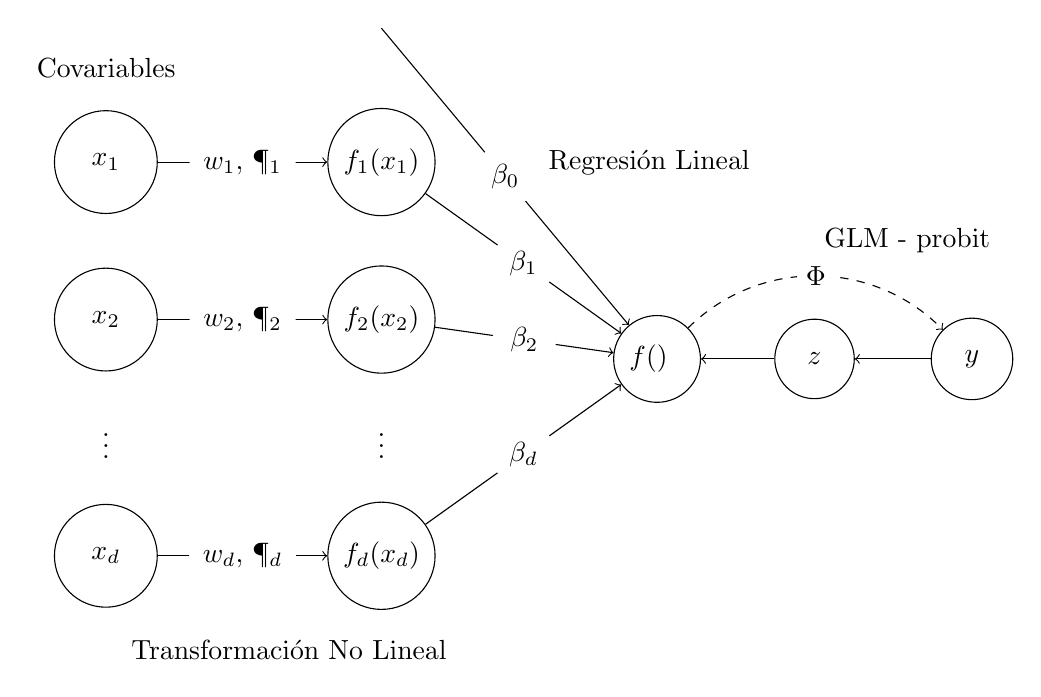
\begin{tikzpicture}

% Nodos Input
\begin{scope}[
		every node/.style = {shape = circle, draw = black,
			minimum size = 10mm,
			text width = 10mm, align = center}]
	\node (x1) at (0,6) {$x_1$};
	\node (x2) at (0,4) {$x_2$};
	\node[draw = white]     at (0,2.5) {$\vdots$};
	\node (xd) at (0,1) {$x_d$};

% Nodos Segunda Capa
	\node (f1) at (3.5,6) {$f_1(x_1)$};
	\node (f2) at (3.5,4) {$f_2(x_2)$};
	\node[draw = white]     at (3.5,2.5) {$\vdots$};
	\node (fd) at (3.5,1) {$f_d(x_d)$};
\end{scope}

% Nodos Lineales
\begin{scope}[
		every node/.style = {shape = circle, draw = black,
			minimum size = 7mm,
			text width = 7mm, align = center}]
\node (f) at (7,3.5) {$f(\xsn)\quad$};
\node (z) at (9,3.5) {$z$};
\node (y) at (11,3.5) {$y$};
\end{scope}

% Nodos Texto 

\node[right] at (-1,7.2) {Covariables};
\node[right] at (0.2,-0.2) {Transformación No Lineal};
\node[right] at (5.5,6) {Regresión Lineal};
\node[right] at (9,5) {GLM - probit};

% Pahts x a f_j y f_j a f
\begin{scope}[
		every node/.style={fill = white, circle},
	    every edge/.style={draw = black, ->}]
	 
	% Paths x a f_j
	\path (x1) edge node {$w_1, \, \P_1$} (f1);
	\path (x2) edge node {$w_2, \, \P_2$} (f2);
	\path (xd) edge node {$w_d, \, \P_d$} (fd);

	% Paths f_j a f
	\path (3.5,7.7) edge node {$\beta_0$} (f);	
	\path (f1) edge node {$\beta_1$} (f);
	\path (f2) edge node {$\beta_2$} (f);
	\path (fd) edge node {$\beta_d$} (f);
\end{scope}

% Ultimos Paths
	\path[->, dashed] (f) edge [bend left = 45]
	node [fill = white] {$\Phi$}(y);	
	\draw[->] (y) -- (z);	
	\draw[->] (z) -- (f);

\end{tikzpicture}
\caption{\textbf{Diagrama del modelo.} Se hace una transformación no lineal de las covariables $x_j$ a través de los parámetros $w_j$ y $P_j$. Con los datos transformados $f_j$, se lleva a cabo un modelo probit con función liga $\Psi$ para lograr la clasificación binaria en $y$.}
\label{fig:DiagramaMod}
\end{figure}

Antes de continuar, vale la pena recordar que:
\begin{quote}
\textit{All models are wrong but some are useful}\footnote{\autocite{box1979robustnessinthe}}
\end{quote}

Escoger un modelo que explique perfectamente los datos o que logre predecir todo sería una tarea inútil. Sin embargo, no significa que no se pueda intentar discernir un patrón y es justamente lo que se busca con la construcción de este modelo. Además de entender a profundidad un modelo que sirve como base para modelos que se están usando en el mundo de la inteligencia artificial. En particular, este modelo tiene la ventaja que es flexible y, al menos en teoría, debería de servir para representar una gran cantidad de datos.

\section{Modelos Lineales Generalizados (GLM)} \label{sec:GLM}
Los Modelos Lineales Generalizados \autocite{sundberg2016exponential} y \autocite{maccullagh1989generalized}, surgen como una generalización flexible del modelo lineal ordinario $y = \beta^tx + \epsilon$ donde $y\in\mathbb{R}$. En esta flexibilización  se busca darle otras distribuciones a $y$ pues tenemos casos donde esta no pertenece a los reales. Sin embargo, este cambio vuel
ve el modelo más complejo y lleva a problemas de estimación de los parámetros. Ade más, se pierde algo de la interpretabiliad del modelo\footnote{Dependiendo de la especificación, su interpretación puede ser complicada. Por ejemplo, cuando se tiene un Modelo Logit tradicional, se logra expresar el logaritmo de la proporción de probabilidades (\textit{Log-Odds-Ratio}) como una combinación lineal de las covariables. $\ln(\pi_i / \pi_0) = \beta^t x$}. Sin embargo, han resultado ser realmente útiles. Los GLM se especifican (de manera muy general) de la siguiente manera:

\begin{align*}
	y &\sim F(\theta(x)) \\
	z &= \beta^tx \\
	\theta &= g^{-1}(z) 
\end{align*}

con los siguientes tres elementos:

\begin{enumerate}
	\item $F$: \textbf{Tipo de distribución} de la familia exponencial para $y$ que trate de describir su dominio. Por ejemplo: Bernoulli si $y$ es binaria, Poisson si $y \in \mathbb{Z}^+$ o una distribución Gamma si $y \in \mathbb{R}^+$
	\item $z$: \textbf{Proyector Lineal} que explique (linealmente) la variabilidad sistemática de tus datos. En el modelo tradicional $\text{dim}(\beta) = d < n.$
	\item $g$: \textbf{Función Liga} que una la media (o los parámetros) $\theta$ de mi distribución con el proyector lineal. Es decir: $\theta(x) = \E[y|x] = g^{-1}(\beta^tx)$. 
	
	Como ejemplos clásicos se tiene la función $\text{logit}(p) = \ln(p/(1-p))$ o la $\text{probit(p)} = \Phi^{-1}(p)$, donde $p = \E[y|x]$ y $\Phi(\cdot)$ es la función de acumulación de una distribución normal estándar. En la Figura \ref{fig:DiagramaFuncLiga} podemos ver una representación gráfica para su mejor comprensión.
\end{enumerate}

% Diagrama de g
\begin{figure}[h]
\centering
\begin{tikzpicture}

% Flechas (circulo) (Solo para demostrar que el orden importa en rikz
%\draw [black] (0,0) circle [radius = 2];

% Dibujo nodos
\begin{scope}[
		every node/.style = {fill = white, shape = rectangle }]
		
	\node (g) at (0,1) {$g$};
	\node (ginv) at (0,-1) {$g^{-1}$};
	\node (R) at (1,0) {$\mathbb{R}$};
	\node (int) at (-1,0) {$[0,1]$};
	
\end{scope}

% Flechitas
\begin{scope}[
		every node/.style={fill = white, circle},
	    every edge/.style={draw = black, ->}]
	
	\path (g) edge [bend left] node [above right] 
	{e.g. $\Phi^{-1}(p)$} (R);
	\path (R) edge [bend left] node [below right] {x} (ginv);
	\path (ginv) edge [bend left] node [below left]
	{e.g. $\Phi(x)$} (int);
	\path (int) edge [bend left] node [above left] {p} (g);
	
\end{scope}

\end{tikzpicture}
\caption{Esquema de función Liga $g$}
\label{fig:DiagramaFuncLiga}
\end{figure}

Para este trabajo, se busca construir un clasificador binario por lo que $y \in \{0,1\}$, por lo cual, es natural modelar $y$ como una distribución Bernoulli. Notese que si $Y \sim \Be(y|p)$ tenemos las siguientes propiedades: 
\begin{align*}
	\E[Y] &= p = P(y = 1) \\
	\Var[Y] &= p(1-p)
\end{align*}

Por lo que solo se tiene un parámetro $p$ y la varianza queda determinada automáticamente. Además, esta especificación deja como  opción para las función liga, a las inversas de las funciones \textit{sigmoidales} $s(x)$. Las funciones sigmoidales, son funciones $s:\mathbb{R}\rightarrow (0,1)$, estrictamente monótonas y por ende, biyectivas. Algunos ejemplos son las ya mencionadas logit, probit y la curva de Gompertz\footnote{Para no caer en redundancia de notación en este trabajo: $s(x) = g^{-1}(x) = \Phi(x)$}. Estas funciones cumplen un papel de activación, es decir, una vez que se rebase cierto umbral, crecen rápidamente y toman valores más cercanos a uno, \textit{activando} asi la probabilidad\footnote{En un contexto de Redes Neuronales, lo que se activa es la neurona y recientemente, se usa la función \textit{ReLu} $(x):= \max\left\{0,x\right\}$}. Esto las hace perfectas herramientas para ligar el proyector lineal $z\in\mathbb{R}$ con una probabilidad $p\in[0,1]$.\\

\subsection{Uso de la Variable Latente}

Ahora para entender el papel que juega $z$, se necesita entender que es posible estructurar estos modelos como \textit{Modelos de Variable Latente} \autocite{albert1993bayesian}. Bajo esta formulación, se asume que la relación entre $y$ y $x$ no es directa, sin embargo, existe una variable no observada $z$ puramente estructural que nos ayuda a discernir un vínculo entre ellas. En la Figura \ref{fig:DiagramaVar} tenemos esa  representación del modelo. \\

%Diagrama de Variable latente
\begin{figure}[h]
\centering
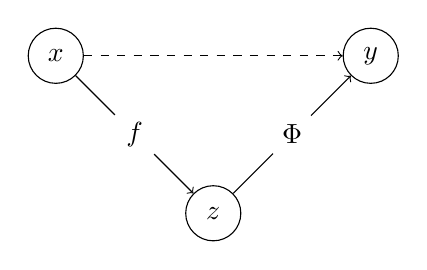
\begin{tikzpicture}

% Nodos Input
\begin{scope}[
		every node/.style = {shape = circle, 
		draw = black, minimum size = .7cm}]
	\node (X) at (0,2) {$x$};
	\node (Y) at (4,2) {$y$};
	\node (Z) at (2,0) {$z$};
\end{scope}

% Paths
\begin{scope}[
		every node/.style={fill = white, circle},
	    every edge/.style={draw = black, ->}]
	\path (X) edge node {$f$} (Z);
	\path (Z) edge node {$\Phi$} (Y);
	\draw[dashed, ->] (X) to (Y);
\end{scope}
\end{tikzpicture}
\caption{Modelo de Variable Latente}
\label{fig:DiagramaVar}
\end{figure}

Tradicionalmente, se asumía normalidad en $z$ derivado de que $z = \beta^tx + e$ con $e \sim N(0,\sigma^2)$, lo cual nos lleva a que $z \sim N(\beta^tx,\sigma^2)$. Además esto facilita la estructura de los modelos y el algoritmo de ajuste\footnote{En el trabajo original, se usa un algoritmo \textit{Gibbs Sampler} con distribuciones truncadas de la normal para encontrar las $\beta$'s}.\\

Para este trabajo se escoge como función liga a la probit $\Phi^{-1}(p)$, es decir la inversa de la función de acumulación normal estándar:

$$\Phi(x) = \int_{-\infty}^x \dfrac{1}{\sqrt{2\pi}}e^{-\frac{t^2}{2}}\, dt$$

La cual claramente es sigmoide. Esta función, cumple el propósito de modelar y cuantificar la incertidumbre pues transformando una variable real $z$ en una probabilidad $p$ con su característica forma de ``s''. Se hace notar que podríamos haber usado una función más flexible o que incluso podríamos haber dejado la función sin especificar, sin embargo, para no complicar más el modelo y poder entender los GLM's a fondo se toma esa decisión. La parte flexible de este modelo se encuentra en el \textit{proyector lineal} que se explica en la Sección \ref{sec:FuncProy}. Con base en esta decisión y el supuesto de que $Y$ es Bernoulli, se deriva la normalidad de $z$ \autocite{albert1993bayesian}; diferente de el enfoque tradición de asumir normalidad en los errores aleatorios\footnote{Este punto de vista, ayuda sobre todo en modelos multinomiales, pues se puede asumir una estructura de inter-dependencia en los errores aleatorios. $\mathbf{e} ~ N_k(0, \Sigma)$ con $\Sigma$ una matriz de correlaciones}.\\

Habiendo definido la función liga, distinguir entre si $y = 1$ ó 0, se reduce a distinguir en que área del espacio de covariables $\mathcal{X}^d$ nos encontramos. Esto se debe a que $y = 1$ cuando $\Phi(z) > 1/2 \iff z>0$ lo cual, dependerá en gran media de la media de $z$ (en este caso $f(\xsn)$). Por lo tanto, es fundamental para el modelo que se realice una correcta estimación de los parámetros de $f(\xsn)$ para que logre separar el espacio de covariables $\mathcal{X}^d$ en los casos donde $y = 1$ y su opuesto. Nótese además, que z le agrega cierta estocasticidad al modelo. Supongamos que existe una pareja $(y_i,\xni)$ tal que $f(\xni) = 0$, alrededor de una vecindad, significaría que no existe evidencia para clasificación a $y_i$ como un éxito o como un fracaso. En ese caso, sería mejor un volado. \\ 

Otro factor importante a considerar también es que nuestro modelo asume $\sigma^2$ desconocida y como un parámetro a estimar (también se maneja de forma bayesiana). Este factor de variabilidad captura las posibles diferencias en escala entre los datos y la variable latente $z$, además de dar cierta flexibilidad a regiones con mucha incertidumbre sobre la clasificación.\\ 

% REVISAR
% Probar (o buscar la prueba de este resultado)
Es importante mencionar, que el \textit{corte} que se hace en 0 para la clasificación, es resultado de hacer una clasificación binaria. En modelos multinomiales también se debe tomar en cuenta los intervalos en $\mathbb{R}$ para los que la observación se clasificaría en alguna de las $k$ clases y por ende, estimar los umbrales o usar una función diferente a las sigmoides. Este hecho, lleva a la realización de que $z$ y su media $f$ son \textit{ajenas más no independientes}. Esto quiere decir que la parametrización de $z$ como una normal $N(\mu,sigma^2)$ es ecuivalente a la parametrización $N(0,1)$. Este hecho se hará más claro cuando hablemos del papel de la $\beta_0$ en la función de proyección. \\ 

Finalmente, si quisiéramos ver la relación directa de $x$ en $y$ directamente, se puede lograr usando el  Teorema de la Probabilidad Total. Se puede calcular (al menos de forma teórica), la distribución marginal de $y$ dado $\xsn$ sumando sobre $z$. Es decir:

% REVISAR
% Integral en libro de Cox
\begin{align*}
P(y|x) 	&= \intinfty P(y|z)P(z|x)\, dz \\
		&= \intinfty p(y;\Phi(z))p(z;f(\xsn),\sigma^2)\, dz \\
		&= \intinfty \Phi(z)^y (1-\Phi(z))^{1-y}
		\dfrac{1}{\sqrt{2\pi\sigma^2}}e^{-\frac{1}{2\sigma^2}(z-f(\xsn))^2} \, dz
\end{align*}

Sin embargo, no lleva a ningún resultado analítico conocido pues la relación es bastante más compleja como para resultar en una distribución  tradicional; si lo hiciera, todo el propósito de la $z$ se perdería.\\

Recapitulando, mediante la función liga $\Phi$ se une la media $p$ de la respuesta $y$ con los datos. Esta función liga se deja rígida y en este trabajo se opta por añadir una nueva capa de complejidad y  flexibilizar el proyector lineal por una función genérica $f$ que se detalla en la siguiente sección. Quedando:

\begin{align} \label{ec:MediaProy}
	P(y = 1) = p(\xsn) &= \theta(\xsn) =\E[y|\xsn] = g^{-1}(f(\xsn)) = \Phi(f(\xsn))
\end{align}

\section{Función de proyección $f$} \label{sec:FuncProy} 
Tradicionalmente, se asumía que $z$ es una combinación lineal de los parámetros $\beta$ y las covariables $x$, pero, como se explica en la pagina 6 de \autocite{james2013introduction}, conforme avanzaron los métodos y el poder computacional disponible se fueron desarrollando técnicas cada vez más poderosas que permitían romper la linealidad. En 1986, Hastie y Tibshirani introducen los Modelos Aditivos Generalizados (GAM), una clase de modelos donde se lleva a romper la linealidad en las covariables, esto permite flexibilizar aún el modelo. Como se vio anteriormente, los GLM siguen la forma especificada en la Sección: \ref{sec:GLM}, sin embargo, al tratar el modelo con la variable latente $z|x \sim N(f(\xsn),\sigma^2)$ con función liga probit, se tiene la ecuación (\ref{ec:MediaProy}).\\

Esta nueva \textit{capa} no hace otra cosa más que ir colapsando dimensiones, ie: $\mathcal{X}^d \rightarrow \mathbb{R} \rightarrow [0,1]$. Es por esto que se llama función de proyección, pues \textit{proyecta} el espacio $\mathcal{X}^d$ en  $\mathbb{R}$. Sin embargo, la forma en la que lo hace debe de ser muy sutil pues el modelo recae en que este colapso detecte los patrones correctos en las covariables que llevan a la correcta identificación de $y$. Por lo tanto, $f$ como función de proyección es el corazón del modelo, por lo que su correcto entrenamiento es fundamental. La idea, recapitulando, es que $f$ separe el espacio de covariables para que sea positiva en las regiones donde tengamos éxitos y negativa donde tengamos fracasos; para ello, es fundamental entender los GAM.\\

\subsection{Modelos Aditivos Generalizados (GAM)} \label{sec:GAM}
Un GAM como lo introducen Hastie y Tibshirani en \autocite{hastie1986generalized} remplaza la forma lineal $\sum_{1}^d\beta_ix_i = \beta^tx$ con una suma de funcione suaves $\sum_i^d f_i(x_i)$. Estas funciones no tienen una forma cerrada y son no especificadas, es decir, no hay tienen una forma funcional concreta y representable algebraicamente. Donde recae la fuerza del modelo, es que se estiman usando técnicas de suavizamiento no paramétricas\footnote{Las técnicas no paraméticas están fuera del alcance de este trabajo. Sin embargo, vale la pena una mención especial por su funcionalidad, practicidad y forma intuitiva, además del sinfín de aplicaciones que tienen. Una guía comprensiva de estas se encuentra en el libro \textit{All of Non-parametric statistics}\autocite{wasserman2007all}.} como lo sería un Suavizamiento Loess. En estos modelos, se asume que por más grande que sea $\mathcal{X}^d$, la relación que existe entre cada una de las dimensiones se puede explicar de manera aditiva. Esta especificación fue revolucionaria pues no solo regresa interpretabilidad al modelo, sino que simplifica la estimación usando técnicas prácticamente automáticas con el algoritmo de \textit{backfitting}. Además, Los GAM, demuestran que son efectivos en descubrir efectos no lineales en las covariables. \\

Para este trabajo, se escoge la ecuación (\ref{ec:fproy}): 
\begin{align*}
	f(\xsn) \approx \sum_{i=0}^d \beta_i f_i(x_i) 
\end{align*}

Esta función se escoge respondiendo a que este modelo, se planea usar para aplicaciones en econometría, donde las dimensiones $i$'s son independientes entre si y corresponden a diferentes \textit{características} o variables con las que se planea modelar la variable de respuesta. Por ejemplo, se puede pensar que cada $x_i \quad \forall i=1,\ldots,d$ como $d$ series de tiempo con las que se planea predecir cuando vender o comprar cierta acción.\\

La $f$ es una versión versión modificada de un GAM tradicional con tres cambios fundamentales. La primera modificación es que estamos ponderando cada $f_i$ por un parámetro $\beta_i$, esto es, para suavizar aún más cada dimensión y captar el patrón general y no tanto los componentes individuales de cada $x_i$. Se puede pensar en cada $f_i$ como una transformación no-lineal de $x_i$ (como lo sería una transformación logarítmica o una transfomación Box-Cox) por lo que se puede dar una interpretación al parámetro $\beta_i$ como el efecto que tiene la dimensión $i$ en particular para el modelo. Se hace notar que se deja espacio para un término independiente $\beta_0$. Por convención $f_0(\cdot) = 1$ por lo que se puede re-expresar la ecuación anterior (\ref{ec:fproy}) como:

$$
f(\xsn) \approx \beta_0 +\sum_{i=1}^d \beta_i f_i(x_i) = \betasn^t F
$$

% Explicar por qué es fundamental
Donde usando notación vectorial $\betasn\in\mathbb{R}^{d+1}$ y $F \in\mathbb{R}^{d+1}$. La inclusión de este parámetro es fundamental para la correcta especificación del modelo pues ayuda a dar un \textit{sesgo o nivel} base contra el cual comparar la suma y escalar la $f$ para que sea compatible con el umbral de corte en $0$ haciendo ecuivalente la parametrización de $z$ con una normal estándar. \\

La segunda modificación, es una más sutil, aunque es muy práctico manejar las $f_i$'s como indeterminadas y estimarlas con procedimientos de suavizamiento no parametricos, también se puede optar por la vía en la que se especifica su forma funcional, no por ello quitandoles flexibilidad. Los detalles de esto lo dejaremos para la Sección \ref{sec:fj} donde se trata de adapart el procedimiento de \autocite{mallik1998automatic}. Esta modificación, obedece a que para ciertas aplicaciones, sirve hacer el modelo paramétrico en donde cada $f_i$ se modela en su expansión de bases y se puede hacer el ajuste con un algoritmo de minimos cuadrados. (Vease Capitulo 9.1 y Ejemplo 5.2.2 de \autocite{hastie2008elements}).\\

La tercera modificación, es que estamos trabajando con una aproximación en vez de una igualdad para $f$. Se hace notar que esta es uno de los supuestos más fuertes del modelo, esto responde a que el \textit{error aleatorio}, sistemático de los datos, está siendo capturado por una aproximación a la $f$ real, dentro de cada una de las $f_i$'s. En la siguiente sección se explora el porqué de esta aproximación usando técnicas de análisis más avanzadas.\\

Imaginar o peor aún, visualizar $f$ es complicado, pero el objetivo es que (si se tienen datos continuos) $f$ agrega los efectos de cada una de las componentes y separa el espacio en regiones de éxitos y fracasos. Es decir, si tenemos puntos en $\mathbb{R}^2$, $f$ se podrá visualizar en $\mathbb{R}^3$ como una serie de picos y valles donde será positiva en caso de ser éxito y negativa en caso contrario.\\

Finalmente, notemos que este modelo se podría confundir con un Modelos en Bases de Funciones Lineales como lo presentado en Capitulo 3 en \autocite{bishop2006pattern} donde se tiene:

\begin{align} 
	f(\xsn) = \beta_0 + \sum_{i = 1}^d\beta_i f_i(\xsn) \label{ec:ExpansionBases1}
\end{align}

La diferencia radica en que cada $f_i$ es función de todas mis covariables en lugar de solo la dimensión $i$. A estas funciones se les conocen como \textit{funciones base} y son lineales en $\beta$, pero no-lineales para $\xsn$. Se hará una exposición más a detalle en la Sección \ref{sec:fj} pero, las posibilidades son ilimitadas para estas funciones, algunos ejemplos son:

\begin{itemize}
	\item \textbf{Bases Gaussianas:}
	 $$f_i(\xsn) = 
	 \exp\left\{-\dfrac{(\xsn - \mu_i)^2}{2s^2}\right\}$$
	\item \textbf{Funciones sigmoidales:} 
	$$f_i(\xsn) = 
	\sigma\left( \dfrac{\xsn - \mu_i}{s} \right)$$
\end{itemize}

Sin embargo, estos son un grupo de modelos completamente diferente cuyas aplicaciones usualmente son en estimación de curvas y no tanto inferencia como lo busca este trabajo.

\section{Funciones $f_i$} \label{sec:fj}

Finalmente se trata la parte más profunda del modelo, las funciones $f_i$  que, como se mencionó anteriormente, son transformaciones no lineales de cada componente $x_i$ que buscan suavizar la nube de datos, para posteriormente sumarlas entre si y dar una medida $f$ que resuma la información. Como se menciona en la introducción de \autocite{hardle2004semiparametric}, el suavizamiento de los datos es central en la estadística inferencial. La idea es extraer la señal entre el ruido y para ello, se intenta estimar y modelar la estructura subyacente. Este suavizamiento, se llevará a cabo usando una \textit{expansión en bases funcionales} como lo visto en la ecuación (\ref{ec:ExpansionBases1}). Toda la siguiente sección se concentra en darle formas funcionales a las $\Psi$'s. Se usa como   referencia el captiulo 5 de \autocite{hastie2008elements}. \\

Una expansión en bases de una función $h:\mathbb{R}^d\rightarrow\mathbb{R}$ es:

\begin{align} 
	h(\xsn) = \sum_{j = 1}^J w_j\Psi_j(\xsn) \label{ec:ExpansionBases2}
\end{align}

Donde, $\Psi_j(\xsn)$ es la $j$-ésima transformación no lineal de $\xsn$ y una vez especificadas y estimadas, el procedimiento (hacia arriba en el modelo) se hace de forma tradicional pues recobra su estructura lineal. Algunos ejemplos son:

\begin{itemize}
	\item $\Psi_j(\xsn) = x_j$ donde $j = 1,\ldots,d$ y se tiene el modelo lineal más sencillo.
	\item $\Psi_j(\xsn) = \ln x_j$ ó $x_j^{1/2}$ donde se tienen transformaciones no lineales en cada una de las covariables.
	\item $\Psi_j(\xsn) = ||\xsn||$ una transformación lineal de todas las covariables.\footnote{Como se vio en la ecuación (\ref{ec:ExpansionBases1})} 
\end{itemize}

Dependiendo del tipo de datos y de aproximación que se busque, puede ser conveniente usar forma sobre la otra; existen muchas más posibles expansiones de bases. Sin embargo, sobre todo cuando se tiene poca o ninguna experiencia con los datos, se busca una representación más flexible (por no decirla ingenua) de estos. El método más común, es tomar una familia de funciones como los son los polinomios por partes o familias de funciones flexibles que logren representar una gran variedad de patrones. En estos métodos, se cuenta con una gran cantidad de funciones base por lo que se requiere controlar la complejidad; las formas más comunes de lograrlo son:

\begin{itemize}
	\item \textbf{Métodos de Restricción}: como los son los métodos aditivos usados en este trabajo.
	\item \textbf{Métodos de Selección}: como lo son los modelos CART y MARS.
	\item \textbf{Métodos de Regularización}: donde se busca controlar los coeficientes, como los son los modelos \textit{Ridge} y  \textit{LASSO}.
\end{itemize}

Simplificando un poco la exposición, por lo pronto, se puede pensar únicamente en funciones reales, por lo que se deja de usar el subíndice $i$ para indicar el componente del vector $\xsn$.\\

Para este trabajo, se aplica el procedimiento de   \autocite{mallik1998automatic}. Los autores presentan un método revolucionario, que permite estimar con un alto grado de precisión relaciones funcionales entre la variable de respuesta $y$ y el regresor $x\in\mathbb{R}$. Se puede pensar que se busca ajustar una curva tradicional. Esto es, para un conjunto de datos $\left\{(x_i,y_i) \right\}_{i = 1}^n$ se plantea el modelo:

\begin{align}
	y_i = h(x_i) + e_i \quad i = 1,\ldots,n \label{ec:EstCurvas}
\end{align}

con las $e_i$ errores aleatorios de media cero. Este método, combina   los procedimientos paramétricos y no paramétricos desarrollados antes para hacer más robusto el algoritmo de \autocite{hastie1986generalized}. La idea, es ajustar un \textit{polinomio por partes} muy flexible. Estos polinomios, se componen de partes de menor orden entre \textit{nodos} adyacentes. La genialidad del su trabajo es que estos nodos, tradicionalmente fijos, se vuelven parámetros a estimar, usando un paradigma bayesiano. Y no solo eso, sino que permiten \textit{aumentar o disminuir el número de nodos} desarrollando un algoritmo Gibbs sampler trans-dimensional. Esta generalización, logra estimaciones tan robustas, que logran aproximar funciones continuas \textit{casi en todas partes}, como lo son la función Doppler, funciones por bloques y funciones con picos pronunciados. \\ 

\subsection{Polinomios por partes y splines} \label{sec:PolisYSplines}

Antes de llegar a estos polinomios tan flexibles, se busca entender que son los polinomios por partes simplificando la exposición de \autocite{wahba1990splines}. Sea $x\in[a,b]\subseteq\mathbb{R}$, se busca separar $[a,b]$ en $J$ intervalos. Por lo tanto, se construye una partición correspondiente $\P = \left\{\t_1,  \t_2,\ldots,  \t_{J-1} \right\}$ tal que $a \leq  \t_1 < \ldots <  \t_{J-1} \leq b$. Estas $ \t$'s son llamadas \textit{nodos}. Se hace notar, que se puede incluir o no la frontera y que a cada intervalo le corresponde una función $\Psi_j$. Con estos nodos, se puede representar a la función global $h$ en su expansión de bases como en la ecuación (\ref{ec:ExpansionBases2}), donde cada $\Psi_j$ es una función que depende de la partición y de $x$. Por ejemplo, se puede pensar en un caso sencillo donde se tiene que $J = 3$ y se quiere ajustar funciones constantes en cada intervalo. Entonces, las funciones base correspondientes serían:

\begin{align*}
	\Psi_1(x,\P) &= I( x <  \t_1) \\
	\Psi_2(x,\P) &= I( \t_1 \leq x <  \t_2) \\
	\Psi_3(x,\P) &= I( \t_2 \leq x ) 
\end{align*}

Con $I(\cdot)$ la función indicadora que vale $1$ si $x$ se encuentra en la región y $0$ en otro caso. Por lo tanto, 

\begin{align*}
		h(x) &= \sum_{j = 1}^J w_j\Psi_j(x) \\
			 &= w_1 I( x <  \t_1) + w_2 I( \t_1 \leq x <  \t_2) + w_3 I( \t_2 \leq x)
\end{align*}

Lo cual es una función \textit{escalonada}, en el sentido de que para cada región de $x$ tenemos un nivel $w_j$.\footnote{Sin entrar en el detalle, usando una función de perdida cuadrática, es fácil demostrar que cada $\hat{w}_j = \bar{x}_j$ es decir, para cada región, el mejor estimador constatne, es el promedio de los puntos de esa región.} Esta aproximación a mis datos podría servir para datos que estén agrupados por niveles, sin embargo, rara vez será ese el caso.\\

Entre cada pareja de nodos, se puede buscar ajustar un polinomio de grado arbitrario. Adicionalmente, se pueden construir polinomios con  restricciones como continuidad en las derivadas, lo cual logra una estimación más robusta. Esta es la magia de los polinomios por partes, que se les puede pedir cuanta \textit{suavidad} queramos, entendido como la continuidad de la K-ésima derivada. Tradicionalmente, se construyen polinomios cúbicos con segunda derivada continua en los nodos. Esto, pues resulta en funciones suaves al ojo humano que logran aproximar una gran cantidad de funciones.

\subsubsection{Orígenes y justificación de su uso}
La palabra \textit{spline}, \footnote{A diferencia de el texto tradicional de \autocite{deboor1978splines}} se usa para designar a este grupo de polinomios por parte. Sin embargom dependiendo de como se definan pueden denotar funciones muy diversas; hasta ahora no hay consenso en la literatura. Para este trabajo se denota a un \textit{spline de grado $M$} como un polinomio por partes de grado $M-1$ con continuidad hasta la $M-2$ derivada. \autocite{wasserman2007all}. Se hace notar, que se tienen definiciónes de splines muy diferentes a las presentadas aquí, todo está en la definición de la partición que además, puede ser tan flexible como se requiera, por ejemplo los B-Splines.\\

Los splines, surgen en \autocite{schoenberg1964spline} donde se plantea el problema: encontrar $h$ en el espacio de Sovolev $W_{M-1}$ de funciones con $M-2$ derivadas continuas y $M$-ésima derivada integrable al cuadrado que minimice:

$$\int_a^b(h^{(m)}(x))^2\,dx$$ 

sujeta a que interpole los puntos, ie: $h(x_i) = h_i \quad i = 1,2,\ldots,n$. Sin embargo, se hace notar que sea como sea la especificación, se tiene un problema con la la naturaleza global de los polinomios, es decir, se necesita controlar lo que pasa más allá de los nodos de la frontera. Por lo que usualmente se escogen condiciones adicionales o linealidad pasando los nodos. En un contexto estadístico, el problema (\ref{ec:EstCurvas}) se puede plantear como encontrar la función $h$ que minimice:

\begin{align}
	\sum_{i=1}^n(y_i - h(x_i))^2 + \lambda\int_a^b (h^{(m)}(x))^2 \, dx \label{ec:SplinesConRegularizacion}
\end{align}

para alguna $\lambda > 0$, donde la solución se demuestra que son \textit{splines naturales} que se estudian más adelante, específicamente \textit{splines cúbicos naturales} si $m = 2\quad (M = 4)$. Cabe mencionar, que esta formulación del problema engloba muchas de técnicas estadísticas interesantes, además de conceptos de optimización. El lector reconocerá que el primer término claramente es la \textit{suma de residuales cuadrados (RSS)} y el segundo término del sumando es un procedimiento conocido como \textit{regularización}. No es el enfoque entrar a detalle en cada uno de estos pues merecen una tesis por si mismas, sin embargo, se definen en el Apéndice \ref{ap:Definiciones}. Por lo pronto, lo esencial, es que al tratar de minimizar el RSS se puede caer en problemas de sobreajuste en donde los parámetros no estén capturando efectos y patrones subyacentes, sino solo estén tratando de seguir los datos. Para compensar, se penaliza el modelo con segundo termino que controla la complejidad del modelo y la suavidad deseada mediante la $\lambda$. Esto se logra, incorporando un termino de penalización el cual crece a medida que $h$ se vuelve más complicada.\footnote{Si el lector tiene una intuición de análisis, notará que integrar la función al cuadrado, corresponde con el producto interno de las funciones pertenecientes al espacio de Hilbert $\mathcal{L}_2([a,b])$. Más detalles de esto en la Sección \ref{sec:Hilbert}} \\

Una vez más, Hastie y Tibshirani, con su modelo aditivo y función de perdida cuadrática con penalización en la segunda derivada:

\begin{align*}
	y &= \sum_{j = 0}^d h_j(x_j) + \epsilon \\	
	\text{RSS}(h_0, h_1, \ldots, h_d) &= \sum_{i = 1}^n[y_i - \sum_{j = 0}^d h_j(x_{ij})]^2 \, + \, \sum_{j = 1}^d\lambda_j 			\int h_j^{''}(t_j) \, dt_j
\end{align*}

más la convención de que $h_0$ es una constant y las $\lambda_j$ los parámetros de suavizamiento, muestran que $h_j \quad j = 1,\ldots,d$ son splines cúbicos. Sin embargo, el modelo no es identificable pues $h_0$ puede ser arbitraria. Por lo que se necesita una restricción adicional para que el mínimo sea único, esta es:

\begin{align}
	\sum_{i = 1}^n h_j(x_{ij}) = 0 \quad \forall j \label{ec:RestriccionGAM}
\end{align}

es decir, las funciones promedian en cero sobre los datos. Lo que nos lleva a que: $h_0 = \bar{y}$. Por lo que si viéramos cada dimensión $j$, tendríamos que las $h_j$ estarían centradas alrededor de la media $\bar{y}$. Además, la implementación de esta formulación, es conocida como \textit{Algoritmo Backfitting} que será revisado en el Capítulo \ref{cap:Algoritmo}. \\

\subsubsection{Formalización matemática de splines}

Retomando la discusión de la página \pageref{sec:PolisYSplines}, se busca definir un polinomio de grado $M-1$ por partes en $J$ intervalos. Tomando una expansión de bases para cada intervalo, como en el ejemplo anterior, el número de funciones base aumenta en $J$ por cada grado que se agregue, dando un total de $J*M$ bases funcionales, y en consecuencia, el mismo número de parámetros por estimar. Esto ocurre porque necesitamos definir $\mathcal{B}_j = \left\{1,x,x^2,\ldots,x^{M-1}\right\}$ para cada $j$. Sin embargo, esto llevaría a polinomios que se comportan de forma independiente en cada intervalo y no se conectan. La primera condición que se le impone es continuidad en los nodos, lo cual  devuelve $J-1$ parámetros que corresponden a los $J-1$ nodos donde se da la continuidad. Cada grado de continuidad en las derivadas que se le pida al polinomio, se restringe el modelo y por ende, el número de funciones bases necesarias a un total de:

\begin{align}
	N^*(M,J,K) = M*J - K*(J-1) \label{ec:NEstrella}
\end{align}

donde $K$ es el número de restricciones para cada nodo ($K \leq M -1)$, definiendo hasta que número de derivada es continua. Independientemente de la base que escojamos, $N*$ será la \textit{dimensión mínima de la base} es decir, el número de funciones necesarias para representar un polinomio en función de $M$ que define su grado, el número de intervalos $J$, por ende el número de nodos y $K$. Por lo pronto, se centra la discusión cuando $K = M - 1$ regresando a la definición de spline: polinomios de grado $M-1$ con continuidad hasta la $M-2$ derivada. Por ende, la dimensión queda: $N^* = M + J - 1$\\

Ahora, para definir la expansión de bases, se define la función auxiliar \textit{parte positiva}:

$$  x_+ = \max\left\{0,x\right\} $$

quedando una expansión en bases truncada:

\begin{align}
	h(x) &= \sum_{i = 1}^{M + J - 1} w_i \Psi_i(x,\mathcal{P}) \nonumber \\ 
 		 &=	\sum_{i = 1}^M w_i \; x^{i-1} + \sum_{i = 1}^{J-1}w_{M+i}\;(x - \t_i)_+^{M-1}	\label{ec:SplineGeneral}
\end{align}

El primer sumando de (\ref{ec:SplineGeneral}), representa el \textit{polinomio base} de grado $M-1$ %baseline,
que afecta a todo el rango. El segundo sumando, está compuesto únicamente de funciones parte positivas que se van \textit{activando} a medida que $x$ se mueve a la derecha y va pasando por los nodos. Estas funciones parte positiva, capturan el efecto de todos los intervalos anteriores que, al combinarlos con el primer sumando definen un polinomio cúbico en todo $[a,b]$. Se hace notar, que esta derivación de las bases, surge cuando se integra un polinomio por partes constante $M-1$ veces. En cada iteración, se juntan las constantes y se integran por si solas, independientemente de los intervalos, lo cual lleva a este \textit{polinomio base}. De forma más explicita, tenemos las bases:

\begin{align*}
	&\Psi_1(x,\mathcal{P}) = 1 \\ 
	&\Psi_2(x,\mathcal{P}) = x \\ 
	& \vdots \\
	&\Psi_M(x,\mathcal{P}) = x^{M-1}\\
	& \quad \quad \quad \text{el \textit{polinomio base}}\\				
	&\Psi_{M + 1}(x,\mathcal{P}) = (x - \t_1)_+^{M-1} \\				
	& \vdots \\
	&\Psi_{M + J - 1}(x,\mathcal{P}) = (x - \t_{J - 1})_+^{M-1} \\
	& \quad \quad \quad \text{la base truncada}		 
\end{align*}

las cuales forman un espacio lineal de funciones $(M + J - 1)$-dimensional.\\

A estos splines, se les conoce como splines cúbicos y son los más usados cuando se buscan funciones suaves.\\ 

A pesar de la utilidad de los splines por su suavidad, todos sufren de problemas más allá del rango de entrenamiento. Su naturaleza global hace que, fuera de la región con nodos, los polinomios crecen o decrecen rápidamente. Por lo tanto, extrapolar con polinomios o splines es peligroso y podría llevar a estimaciones erróneas. Para corregir esto, en ocasiones, se puede imponer la restricción de que el polinomio deba ser lineal más allá de los nodos frontera. Para designarlos, se les agrega el adjetivo de \textit{natural}. Esta modificación, libera $2*(M-2)$ funciones bases, pues quita todas las bases de orden mayor a 1 en los dos nodos frontera. Adicionalmente, es razonable que se mejore la fuerza predictiva fuera de el dominio de entrenamiento. Todo depende de los datos y el tipo de funciones que se esté tratando de estimar. Su expansión en bases, también se deriva de la ecuación (\ref{ec:SplineGeneral}).\\

Hasta ahora, se han usando los parámetros $M,\;J$ y $K$ para definir el número de funciones base $N^*$, ecuación (\ref{ec:NEstrella}), pero también, sirven para definir los \textit{grados de libertad} que se tienen. Esto se debe a que no solo nos dicen el número de funciones bases y la dimensión del espacio lineal, sino que nos indican el número de parámetros $w_j$'s a estimar. \\

Otra consideración, es que, al estar trabajando en espacios funcionales, la elección de base es relativamente arbitraria y podemos intercambiarla como lo haríamos con una transformación de coordenadas en un espacio euclidiano. Cada base tiene sus beneficios y simplicidad. Aquí se escoge una expansión de bases truncadas pues es explicada fácilmente y tiene una forma funcional relativamente sencilla. Sin embargo, no es óptima computacionalmente cuando $J$ es grande. En la practica, usualmente se implementan B-Splines\footnote{Vease el Capítulo 5.5 de \autocite{wasserman2007all} o el Apéndice del Capítulo 5 en \autocite{hastie2008elements}} que se derivan de los vistos anteriormente.  

\subsection{Polinomios por parte flexibles}

Independientemente de la selección de parametros en la construcción del polinomio, se tiene el problema de la selección de los nodos. Existen procedimientos adaptativos, como los propuestos en \autocite{friedman1991multivariate}. Sin embargo, y como ya se mencionó más atrás, en 1998, Denison, Mallik y Smith proponen un método bayesiano más atractivo.\\

Para poder explicar su método, se tiene que hacerle una modificación a la ecuación (\ref{ec:SplineGeneral}) para convertirla, de un spline, a un polinomio por partes más general con grado arbitrario de continuidad en las derivadas. En su expansión de bases se tiene:

\begin{align}
	h(x) &= \sum_{i = 1}^{N^*} w_i^* \; \Psi_i(x,\mathcal{P}) \qquad \text{con  } N^* = J*M - K*(J-1) \label{ec:ExpBase_wEstrella} \\ 
 		 &=	\sum_{i = 1}^M w_{i,0} \; x^{i-1} + 
			\sum_{i = K}^{M-1} \;
	 		\sum_{j = 1}^{J-1}w_{i,j}\;(x - \t_j)_+^{i}
	 			\label{ec:PoliMallik}
\end{align}

Dado que se tiene una doble suma, es necesario incluir un segundo índice, al menos temporalmente, a los pesos. De, modo que el primer índice, denotado por $i$ refleja el grado asociado a su término\footnote{Desgraciadamente y para ser consistentes con la notación anterior, no se puede indexar directamente, es decir, se le tiene que restar 1 para obtener el grado en los primeros terminos, pero en los posteriores si es directo.}. Por lo tanto, si $i = 2$ entonces, $w_{2,j}$ está asociado a una término de grado 1. El segundo índice $j$ denota al nodo al que está asociado el peso. Como convención, si $j = 0$, se hace referencia al \textit{polinomio base} que siempre tendrá efecto. En el segundo sumando de (\ref{ec:PoliMallik}) la primera suma comienza en $K$. Recordando, $K$ es el número de restricciones de continuidad que se imponen al polinomio en los nodos. Por ejemplo, $K = 0$ implicaría que cada polinomio es independiente; $K = 2$, se tiene continuidad en la función y en la primera derivada, etc. En el caso de que $K = M-1$ regresamos a la ecuación (\ref{ec:SplineGeneral}) y tenemos una vez más splines que, por construcción, son suaves. La suavidad, aunque importante, no siempre es requerida. Existen muchas funciones con primera y segunda derivada que varían rápidamente e incluso funciones discontinuas que no se podrían estimar usando splines; todo depende de los datos. Esta constucción, con su doble suma, permite tener $M-K$ términos por nodo, codificando así las continuidades en las derivadas\footnote{Esta codificación es sutil pues, al hacer los cálculos de continuidad, tenemos que considerar los límites izquierdos y derechos, los cuales existen siempre. Sin embargo, los términos $(x-\t)^K_+$ se desvanecen únicamente hasta la $K$-esima derivada. Para la $(K+1)$-derivada, el coeficiente correspondiente se suma a la función y rompe la continuidad pues no corresponde con el límite izquierdo}. En la ecuación (\ref{ec:ExpBase_wEstrella}) se usa $w_i^*$ solamente para denotar que se puede seguir expresando como una combinación lineal. Finalmente, hágase que $h(x)$ sea igual a $f_i(x_i)$. Con este cambio de notración,(\ref{ec:ExpBase_wEstrella}) es equivalente a (\ref{ec:fj}). Este era el último componente fundamental por definir del modelo, completando así su exposición.\\

En la Figura \ref{tab:Biyeccion} de la página \pageref{tab:Biyeccion}, se hace un compendio de los polinomios por partes. Esto ayuda no solo a esclarecer las cosas, sino a formar una biyección entre $w_i^*$, $w_{n,m}$ y $\Psi_i$ que posteriormente ayudará a expresar todo de forma matricial en su implementación en código.

\begin{figure}[] 
\centering
\renewcommand{\arraystretch}{1.3}
$\begin{array}{l|c|lcc}
w^*_j 				& w_{n,m} 	& \Psi_j(x,\P) 			& ~ & ~ \\[3pt] 
\text{Subíndice } j &\text{Subíndices } n,m & \text{Función Base} & ~ & ~ \\ 
\cline{1-3}
1 					& 1,0 		& 1 					& \rdelim\}{4}{40pt}[$M$ elementos]		 	& ~ \\
2 					& 2,0 		& x 					&											& ~ \\ 
\vdots 				& \vdots 	& \vdots		 		& 											& ~ \\ 
M 					& M,0 		& x^{M-1} 				& 											& ~ \\ 
\cdashline{1-3}
M+1 				& K,1 		& (x-\t_1)^K_+ 			& \rdelim\}{4}{40pt}[$M-K$]		 			& \rdelim\}{13}{50pt}[$J-1$ veces] 	\\ 
M+2					& K+1,1 	& (x-\t_1)^{K+1}_+ 		& 											& 									\\ 
\vdots 				& \vdots	& \vdots 				& 											& 									\\ 
M+(M-K)	 			& M-1,1 	& (x-\t_1)^{M-1}_+ 		& 											& 									\\ 
\cdashline{1-3}
M+(M-K)+1 			& K,2  		& (x-\t_1)^K_+ 	   		& \rdelim\}{4}{40pt}[$M-K$]					& 									\\ 
M+(M-K)+2 			& K+1,2  	& (x-\t_1)^{K+1}_+		&  											& 									\\ 
\vdots 				& \vdots 	& \vdots 				&  											& 									\\ 
M+2(M-K) 			& M-1,2  	& (x-\t_1)^{M-1}_+		& 											& 									\\ 
\cdashline{1-3}
\vdots 				& \vdots 	& \vdots 				& 											& 									\\ 
\cdashline{1-3}
M+(J-2)(M-K)+1 		& K,J-1		& (x-\t_{J-1})^K_+ 	  	& \rdelim\}{4}{40pt}[$M-K$]  				& 									\\ 
M+(J-2)(M-K)+2 		& K+1,J-1 	& (x-\t_{J-1})^{K+1}_+ 	& 											& 									\\ 
\vdots 				& \vdots	& \vdots 				& 											& 									\\ 
M+(J-1)(M-K) 		& M-1,J-1	& (x-\t_{J-1})^{K+1}_+	&  											&  
\end{array}$
\caption{Biyección entre $w_j^*$, $w_{n,m}$ y sus correspondientes funciones base $\Psi_j	$}
\label{tab:Biyeccion}
\end{figure}

Por lo tanto, se termina teniendo $N^* = M + (J-1)(M-K) = JM - K(J-1)$ términos una vez más. Y por construcción, como se vio anteriormente, la biyección, es consistente con la definición en (\ref{ec:SplineGeneral}) para el caso especifico que $K = M-1$. \\

Antes de cerrar el capítulo, se centra la atención en los nodos $\t$. A estos, se les ha dado poca importancia hasta el momento, pues se han considerado como fijos. Como ya se mencionó antes, en \autocite{mallik1998automatic} se desarrolla, además de la ecuación (\ref{ec:PoliMallik}) un paradigma bayesiano para que los nodos, sean tratados como parámetros y por ende sus posiciones son variables. La ventaja de que estos estén indeterminados, es que se pueden concentrar en los lugares donde la función varia más. Y al contrario, si la función es relativamente plana para alguna sección, se necesitan pocos nodos. En el Capitulo \ref{cap:Bayes}, se continua con esta exposición y se detalla el proceso para la selección de la posición de los nodos. Sin embargo, cabe recalcar que a diferencia del trabajo original donde el número de nodos era variable, en este trabajo se usa $J$ fija. Esto corresponde a que se busca simplificar el algoritmo sin tener que usar métodos que aumenten o disminuyan el número de dimensiones. En la practica, la $J$ se tiene que calibrar, sin embargo, no ha resultado ser un problema adicional pues normalmente, se busca suavizar más que estimar estimar funciones especificas complejas como era el objetivo del trabajo original.

\subsubsection*{Consideraciones finales}

Al tener en mente que se tienen $d$ covariables, y por ende $d$ polinomios por partes, además de la estructura lineal de (\ref{ec:ExpBase_wEstrella}) podemos sustituir (\ref{ec:fj}) dentro de (\ref{ec:fproy}) y se tiene la siguiente estructura con doble suma:

\begin{align*}
	f(\xsn) &\approx \sum_{i=0}^d \beta_i f_i(x_i) \\
			&\approx \beta_0 + \sum_{i=1}^d \beta_i \left[\sum_{j=1}^{N^*} w_{i,j}\Psi_{i,j}(x_i, \P_i)\right]
\end{align*}

Lo cual, es perfectamente lineal. Se tienen $1 + d*N^*$ términos y se pueden acomodar en un solo vector. Sin embargo, se tiene un cruce de parámetros interesante, la multiplicación de la $\beta_i\quad \forall i$ contra $w_{i,j} \quad \forall j$. Tradicionalmente, no se usan $\beta$'s y se deja que se capture ese efecto dentro de las $f_i$ como en los modelos aditivos normales. Sin embargo, dado que el objetivo de este trabajo es la predicción, más que la estimación de funciones, se opta por dar una nueva capa de suavizamiento con las $\beta$'s. No existe forma de garantizar ortogonalidad de las $\beta$'s contra las $w$'s, por lo tanto, se le da prioridad a la correcta estimación de $w$ pues captura un mayor efecto además de que, por construcción de los polinomios por partes, si está garantizada la ortogonalidad contra las funciones bases $\Psi$'.

\end{document}

